%!TEX root = ../my_thesis.tex
\chapter{Décodeurs polaires déclenchés par transport} % (fold)
\label{chap:tta}

\vspace*{\fill}
\minitocTITI
\vspace*{\fill}
\newpage

\section*{Introduction}



\section{Transport Triggered Architectures}
Au cours de ce manuscrit, du point de vue de l'architecture des processeurs, deux types de parallélisme ont été abordés.
Le premier est le parallélisme de données.
Pour exploiter ce parallélisme, les jeux d'instructions de certains processeurs incluent des instructions vectorielles SIMD.
C'est le cas des architectures ARM ou x86 actuelles qui incluent respectivement les jeux d'instructions NEON et AVX utilisés dans le Chapitre \ref{chap:soft_scl}.
Les instructions spécialisées de l'ASIP proposé dans le Chapitre \ref{chap:tensilica} sont également des instructions SIMD.
Ces instructions permettent d'appliquer parallèlement une même opération sur plusieurs données.

Le second type de parallélisme est le parallélisme d'instructions. Contrairement au parallélisme de données, il s'agit d'exécuter plusieurs opérations différentes sur plusieurs données d'entrées. Par exemple, effectuer une somme de deux données et, en parallèle, effectuer une opération \textit{ou-exclusif} sur deux autres.
Il existe plusieurs façons de concevoir un processeur permettant du parallélisme d'instructions. Le compilateur peut selon les cas être impliqué dans la détection et l'exploitation du parallélisme d'instructions.

Dans les architecture superscalaires, le compilateur n'est pas impliqué dans la gestion du parallélisme d'instructions. Celui-ci est détecté par des unités matérielles spécialisées. 
Elles permettent de lancer l'exécution de plusieurs opérations parallèles sur les multiples unités fonctionnelles du processeur.
Pour cela, ces unités ont la capacité d'analyser les dépendances entre les données, de changer dynamiquement l'ordre d'exécution des instructions, ainsi que de spéculer sur les futures instructions du programme exécuté. 
Un des avantages de ce type de processeurs est que des programmes séquentiels d'architectures plus anciennes peuvent être accélérés dans nouvelle compilation. Le désavantage est le complexité accrue du processeur causée par l'ajout des unités matérielles responsables de la mise en œuvre du parallélisme. La surface du circuit augmente ainsi que sa consommation énergétique.

Au contraire, dans les architectures dites \og à très long mot d'instruction \fg (VLIW : Very Large Instruction Word), l'essentiel de l'effort nécessaire à la mise en œuvre du parallélisme d'instructions est pris en charge par le compilateur. Le compilateur décrit quelles instructions doivent être exécutées en parallèle, et dans quel ordre. L'avantage des architectures VLIW par rapport aux architectures superscalaires est la réduction de la complexité de la logique de contrôle. De plus, les possibilité de parallélisme d'instructions sont plus facilement identifiées par les compilateurs qui ont une vue plus large du programme que les unités matérielles de parallélisation des architectures superscalaires.

L'architecture du processeur proposé dans ce chapitre fait partie de la famille des architectures déclenchées par le transport (TTA : Transport Triggered Architecture). Les TTAs sont des architectures modulaires particulières proches des architectures VLIW. La principale différences entre les architectures TTA et les architectures VLIW 



\subsection{Principes}


\begin{figure}
\centering
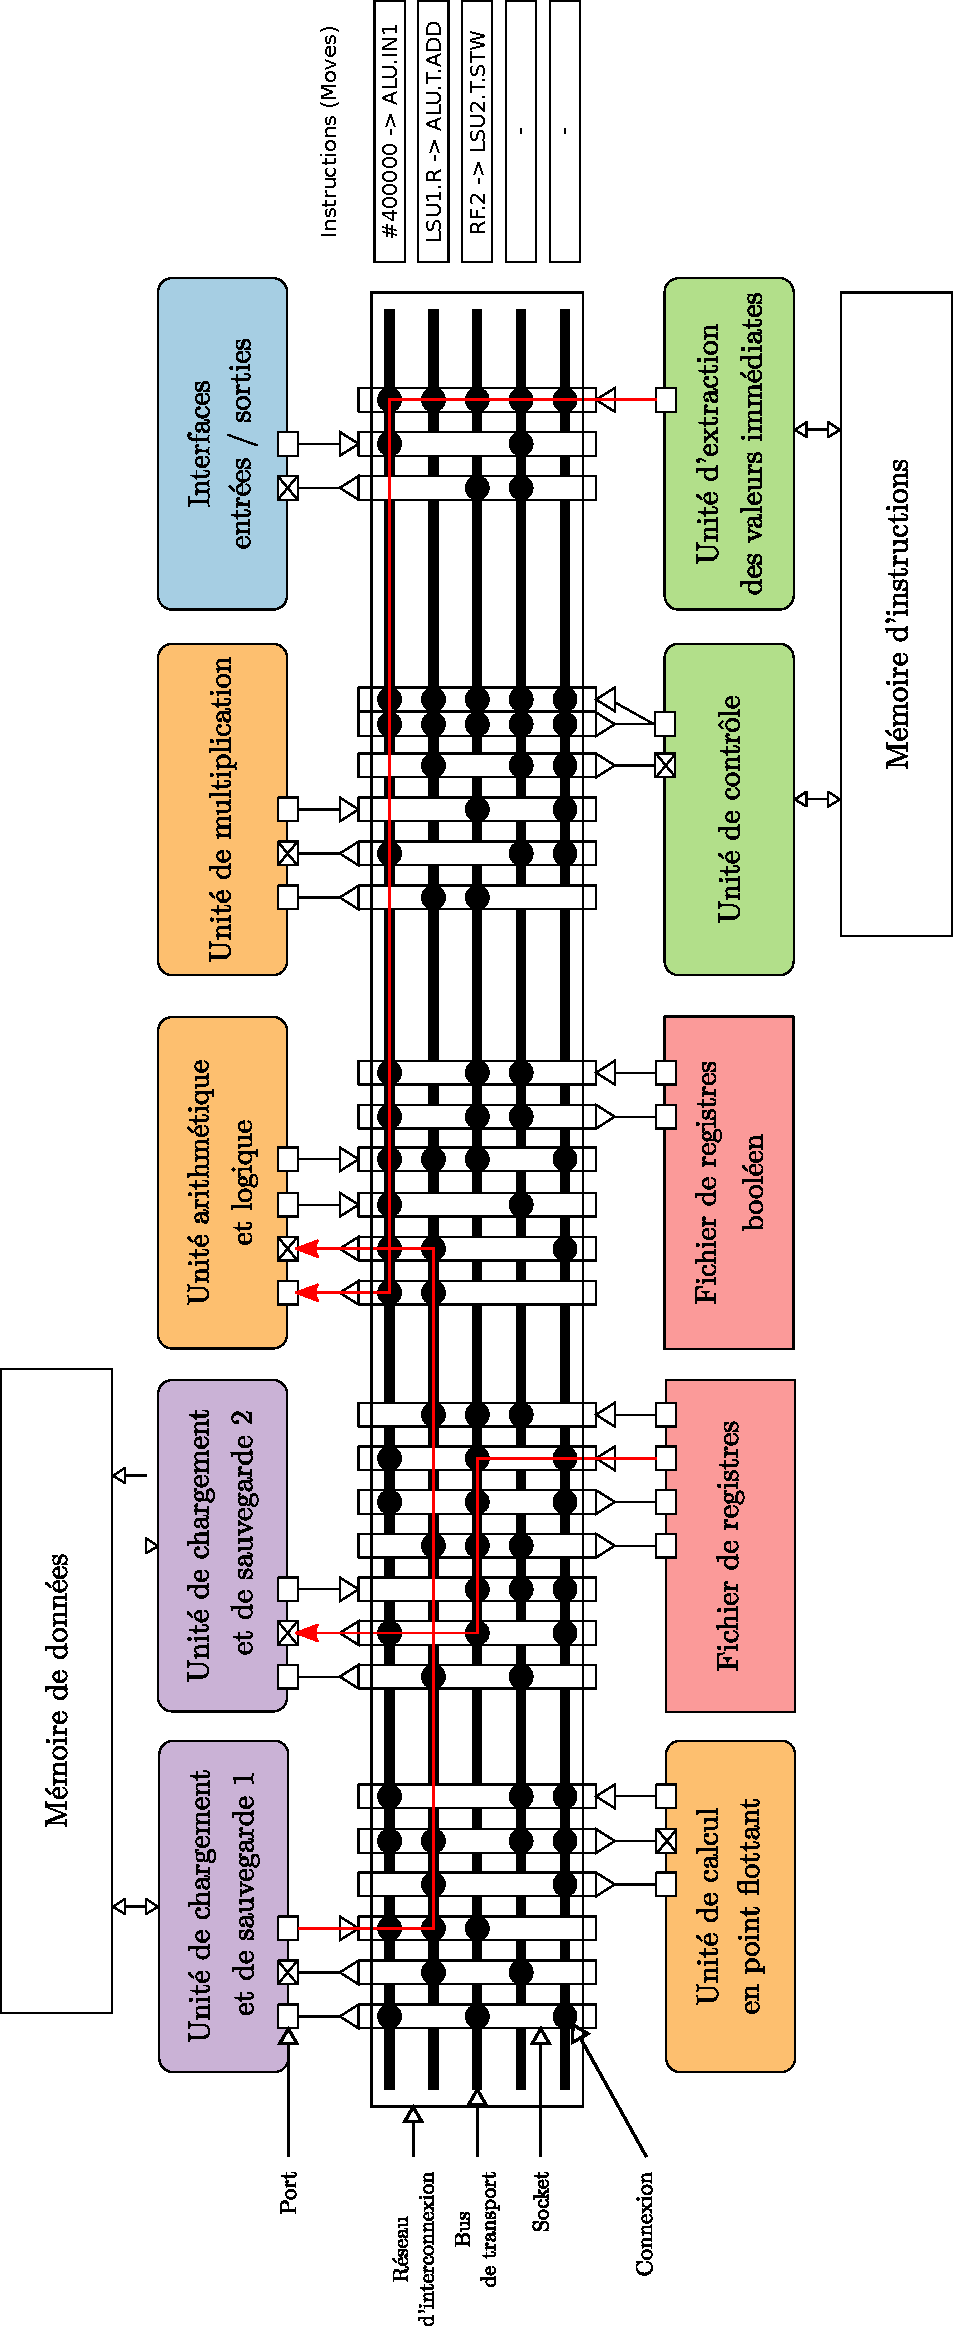
\includegraphics[width=\textwidth]{main/ch4_fig/archi_tta}
\caption{Un exemple d'architecture de processeur TTA. }
\end{figure}
\subsection{Environnement TCE}

\section{Transport Triggered Polar Decoders}

\subsection{Architecture du décodeur SC}
\subsection{Description logicielle}
\subsection{Implémentation de l'algorithme SCAN}

\section{Un flot de conception complet}

\subsection{Génération des vecteurs de tests}
\subsection{Cycles de conception}

\section{Expérimentations et mesures}

\subsection{TT-SC}
\subsection{TT-SCAN}


\section*{Conclusion}


